\documentclass[12pt,a4paper]{article}

\usepackage[utf8]{inputenc}
\usepackage[T2A]{fontenc}
\usepackage[ukrainian]{babel}

\usepackage{geometry}
\geometry{left=2cm,right=2cm,top=2cm,bottom=2cm}

\usepackage{graphicx}
\usepackage{array,multirow}
\usepackage{booktabs}
\usepackage{caption}
\renewcommand{\thetable}{№\arabic{table}}
\captionsetup[table]{name=Таблиця}

\usepackage{amsmath}
\usepackage{pdflscape}
\usepackage{xcolor}

\usepackage{hyperref}

\begin{document}

    \begin{titlepage}

        % Картинка шапки (по центру, з відступом від верху)
        \begin{center}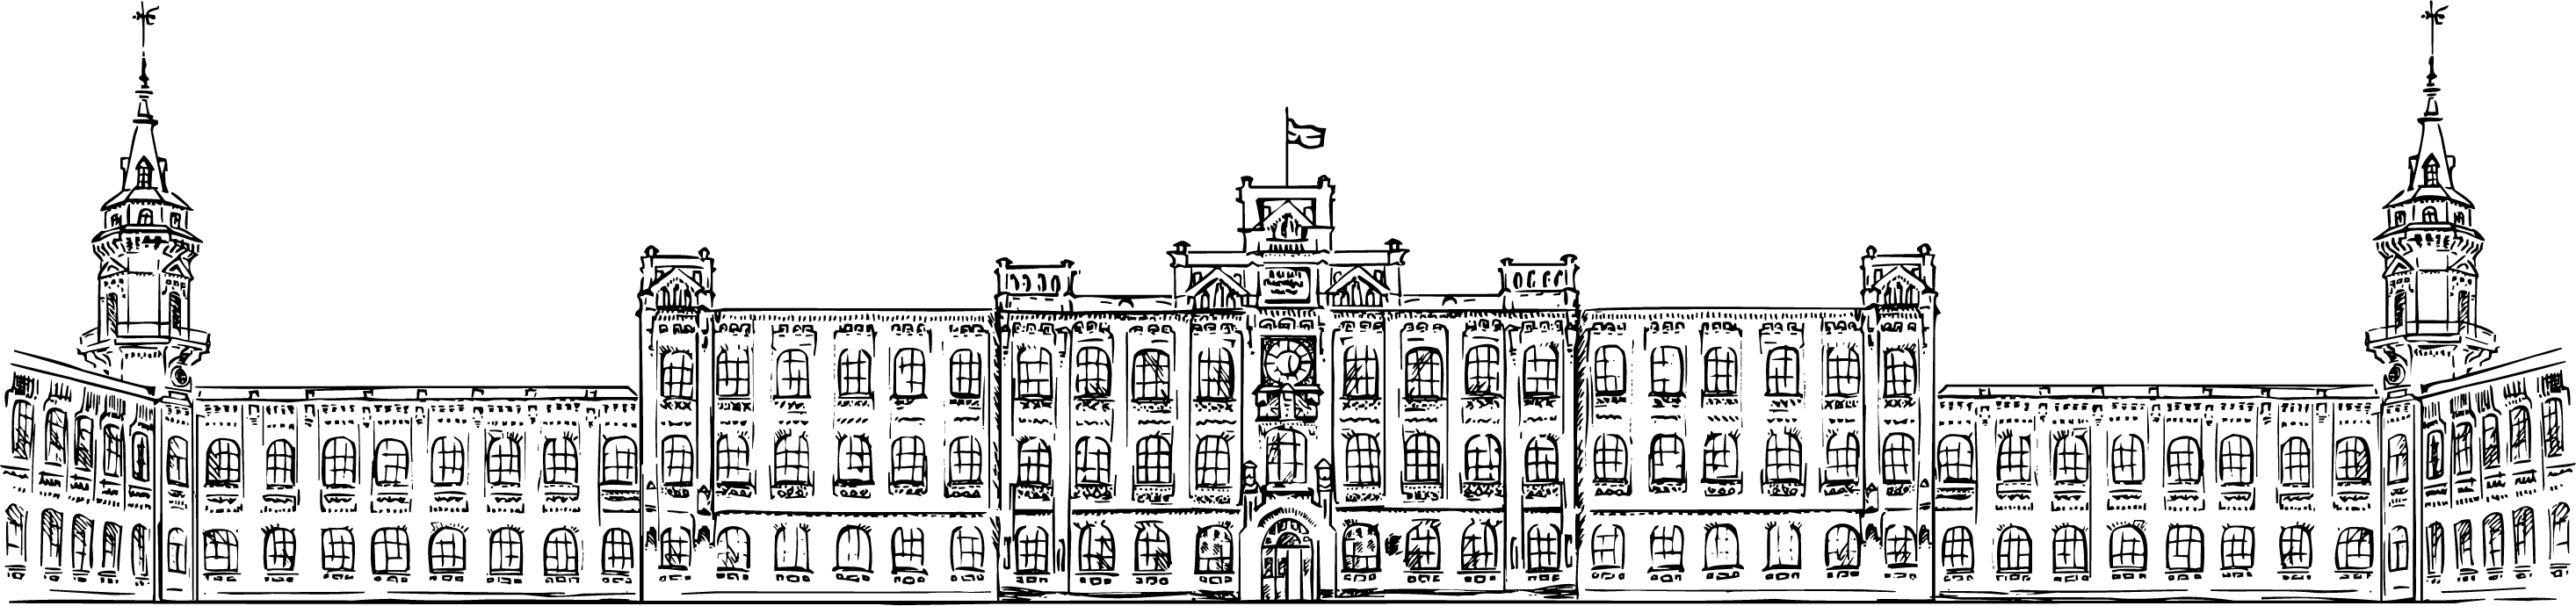
\includegraphics[width=0.7\textwidth]{../../../TITLES/letterhead.png}\end{center}

        \begin{center}
            \large Національний технічний університет України\\
            «Київський політехнічний інститут імені Ігоря Сікорського»\\[1em]
            Факультет інформатики та обчислювальної техніки\\
            Кафедра обчислювальної техніки
        \end{center}

        \vfill

        \begin{center}
            \textbf{\LARGE Практична електроніка}\\[2em]
            \textbf{\Large Лабораторна робота №1}\\
            «Біполярні та польові транзистори»
        \end{center}

        \vfill

        \begin{flushright}
            Виконав: студент 2 курсу ФІОТ, гр. ІО-41\\
            \textit{Давидчук А.~М.}\\[1em]
            Перевірив: \textit{Гайдай А.~Р.}
        \end{flushright}

        \vfill

        \begin{center}Київ --- 2025\end{center}

    \end{titlepage}

    % Основний документ:

    \setlength{\parindent}{0em}

    \textbf{\underline{Тема:}} «Біполярні та польові транзистори».
    
    \vspace{1em}

    \textbf{\underline{Мета:}} Дослідити принцип дії та основні властивості біполярних (БТ) та
    польових транзисторів (ПТ); дослідити основні динамічні характеристики БТ, які
    включено за схемою зі спільним емітером (СЕ); ознайомитися з основними
    параметрами цих пристроїв та областю їх застосування.

    \begin{center} \textbf{\Large Практична частина} \end{center}

    Мій порядковий номер у списку: 6. Звідси визначу, що $F = 6$.

    \setlength{\parindent}{1.5em}

    \begin{center} \textbf{\large Аналіз схеми №1} \end{center}

    \begin{figure}[h!]

        \renewcommand{\thefigure}{\arabic{figure}} % робимо "3.1", "3.2" і т.д.

        \centering
        % Підставляєте потрібний шлях та розмір зображення:
        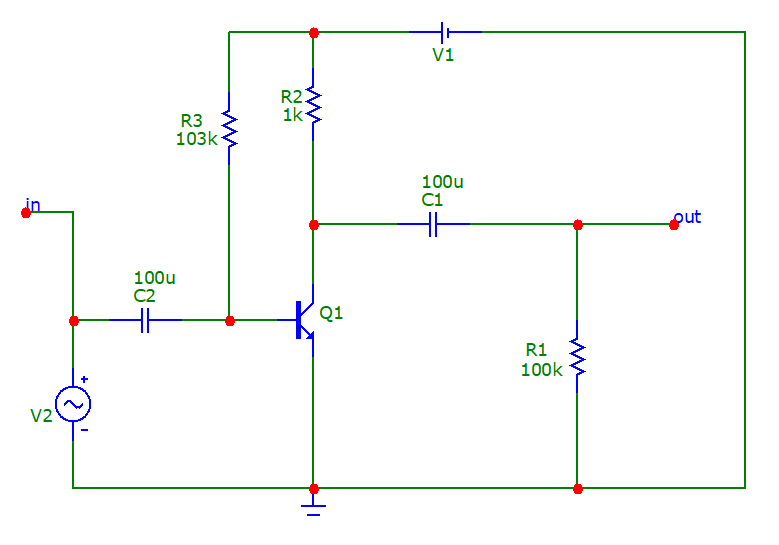
\includegraphics[width=0.5\textwidth]{scheme1-1.png}
        % Підпис (зазвичай під малюнком):
        \caption{\centering Схема однокаскадного підсилювача із фіксованим базовим струмом на біполярному n-p-n-транзисторі}
        % Мітка для посилань у тексті (\ref{fig:...})
        \label{fig1-1:schema}

    \end{figure}

    \begin{figure}[h!]

        \renewcommand{\thefigure}{\arabic{figure}} % робимо "3.1", "3.2" і т.д.

        \centering
        % Підставляєте потрібний шлях та розмір зображення:
        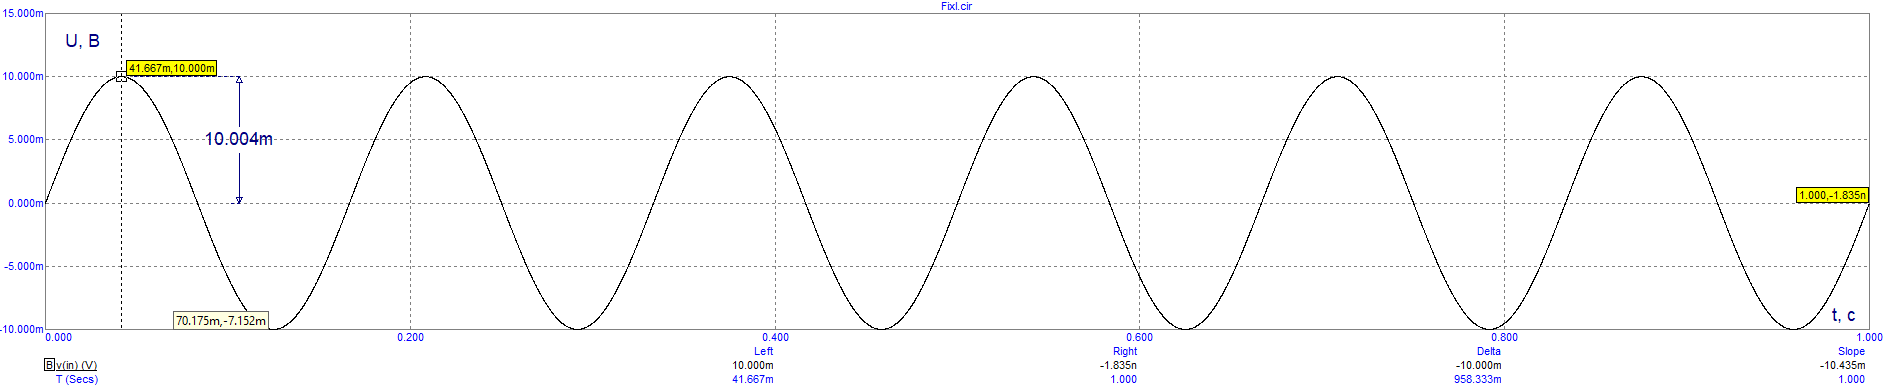
\includegraphics[width=0.7\textwidth]{graph1-2-1.png}
        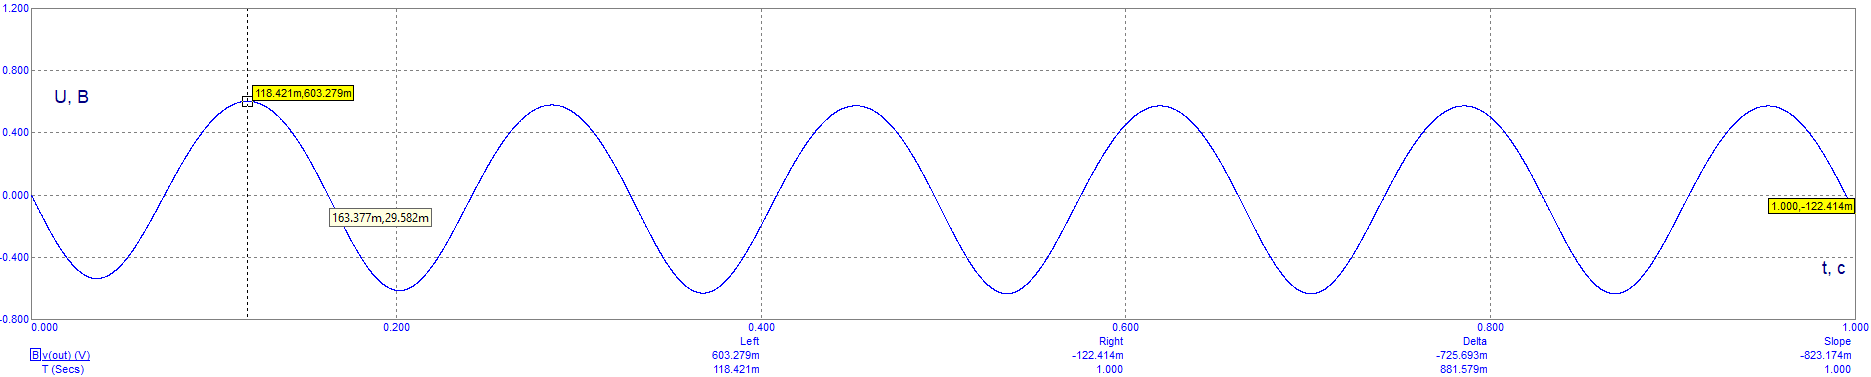
\includegraphics[width=0.7\textwidth]{graph1-2-2.png}
        % Підпис (зазвичай під малюнком):
        \caption{Часові діаграми роботи схеми з фіксованим струмом бази (вхід та вихід)}
        % Мітка для посилань у тексті (\ref{fig:...})
        \label{fig1-2:graph}

    \end{figure}

    Як видно із часових діаграм: вихідний сигнал був інвертований, та підсилений. І, відповідно, ми можемо обчислити коефіцієнт підсилення:

    \[
    K = \frac{U_{out}}{U_{in}} = \frac{603{,}279 \cdot 10^{-3}}{10\cdot 10^{-3}} \approx 60{,}33
    \]

    Під час моделювання підсилювача з фіксованим струмом бази було встановлено, що схема забезпечує одночасно підсилення та інверсію сигналу.
    При вхідній напрузі $\approx10$ мВ вихідна досягла $\approx603$ мВ, що свідчить про значне збільшення амплітуди. Зафіксований зсув фази на 180° підтверджує властивості підсилювача із загальним емітером і правильність вибраного режиму роботи.

    Зробимо розрахунок для даної схеми, тим самим перевіривши значення вибраного для досліду опору бази.

    \newpage

    \begin{figure}[h!]

        \renewcommand{\thefigure}{\arabic{figure}} % робимо "3.1", "3.2" і т.д.

        \centering
        % Підставляєте потрібний шлях та розмір зображення:
        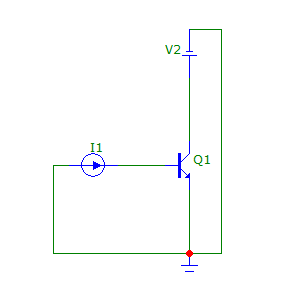
\includegraphics[width=0.5\textwidth]{scheme1-2.png}
        % Підпис (зазвичай під малюнком):
        \caption{\centering Схема для побудови вхідних характеристик транзистора 2N699}
        % Мітка для посилань у тексті (\ref{fig:...})
        \label{fig1-2:schema}

    \end{figure}

    \begin{figure}[h!]

        \renewcommand{\thefigure}{\arabic{figure}} % робимо "3.1", "3.2" і т.д.

        \centering
        % Підставляєте потрібний шлях та розмір зображення:
        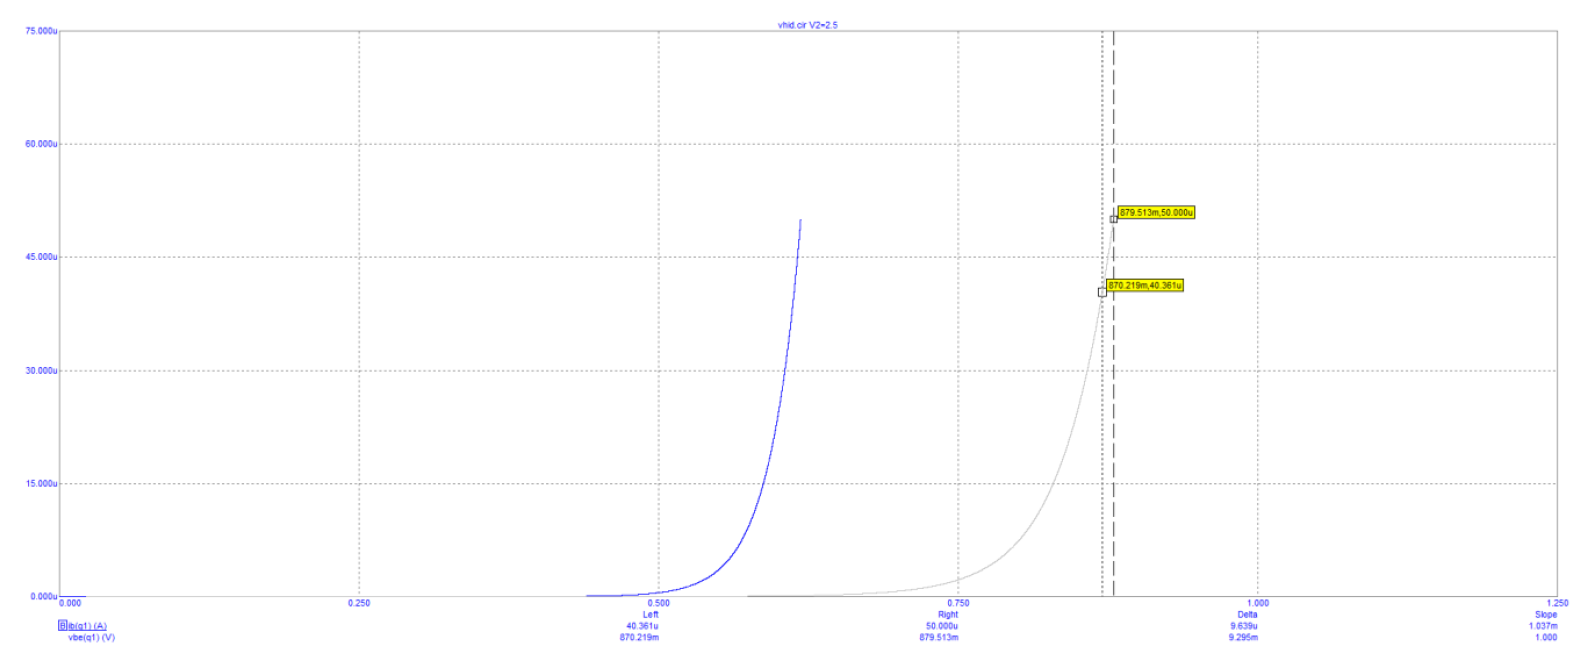
\includegraphics[width=0.9\textwidth]{graph1-3.png}
        % Підпис (зазвичай під малюнком):
        \caption{Вхідні характеристики транзистора 2N699}
        % Мітка для посилань у тексті (\ref{fig:...})
        \label{fig1-3:graph}

    \end{figure}

    Тут $I_{\text{бо}} = 40$ мкА, $U_{\text{беО}} = 870{,}219$ мВ, $E_{\text{к}} = 5$ В. І обчислимо опір бази за формулою

    \[
    R_{\text{б}} = \frac{E_{\text{к}} - U_{\text{беО}}}{I_{\text{бо}}} = \frac{5 - 870{,}219 \cdot 10^{-3}}{40 \cdot 10^{-6}} \approx 103 \cdot 10^3 \text{ Ом}
    \]

    На графіку наведено вхідну характеристику біполярного n-p-n транзистора 2N699, що відображає залежність струму бази від напруги між базою та емітером.
    За малих значень напруги струм практично відсутній, проте після досягнення $\approx0{,}87$ В він різко зростає, що свідчить про відкриття p-n переходу
    й перехід транзистора в активний режим. Позначені точки на кривій використовуються для визначення робочої точки підсилювача та подальших розрахунків параметрів кола,
    зокрема елементів базового кола.

    Для визначення опору на колекторі, необхідно скористатися графіком вихідних характеристик.

    \newpage

    \begin{figure}[h!]

        \renewcommand{\thefigure}{\arabic{figure}} % робимо "3.1", "3.2" і т.д.

        \centering
        % Підставляєте потрібний шлях та розмір зображення:
        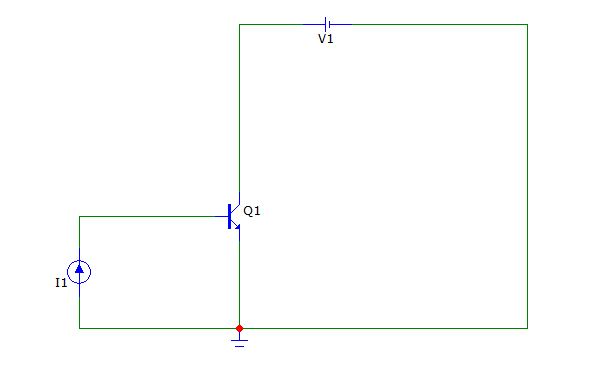
\includegraphics[width=0.5\textwidth]{scheme1-3.png}
        % Підпис (зазвичай під малюнком):
        \caption{\centering Схема для побудови вихідних статичних характеристик транзистора 2N699}
        % Мітка для посилань у тексті (\ref{fig:...})
        \label{fig1-3:schema}

    \end{figure}

    \begin{figure}[h!]

        \renewcommand{\thefigure}{\arabic{figure}} % робимо "3.1", "3.2" і т.д.

        \centering
        % Підставляєте потрібний шлях та розмір зображення:
        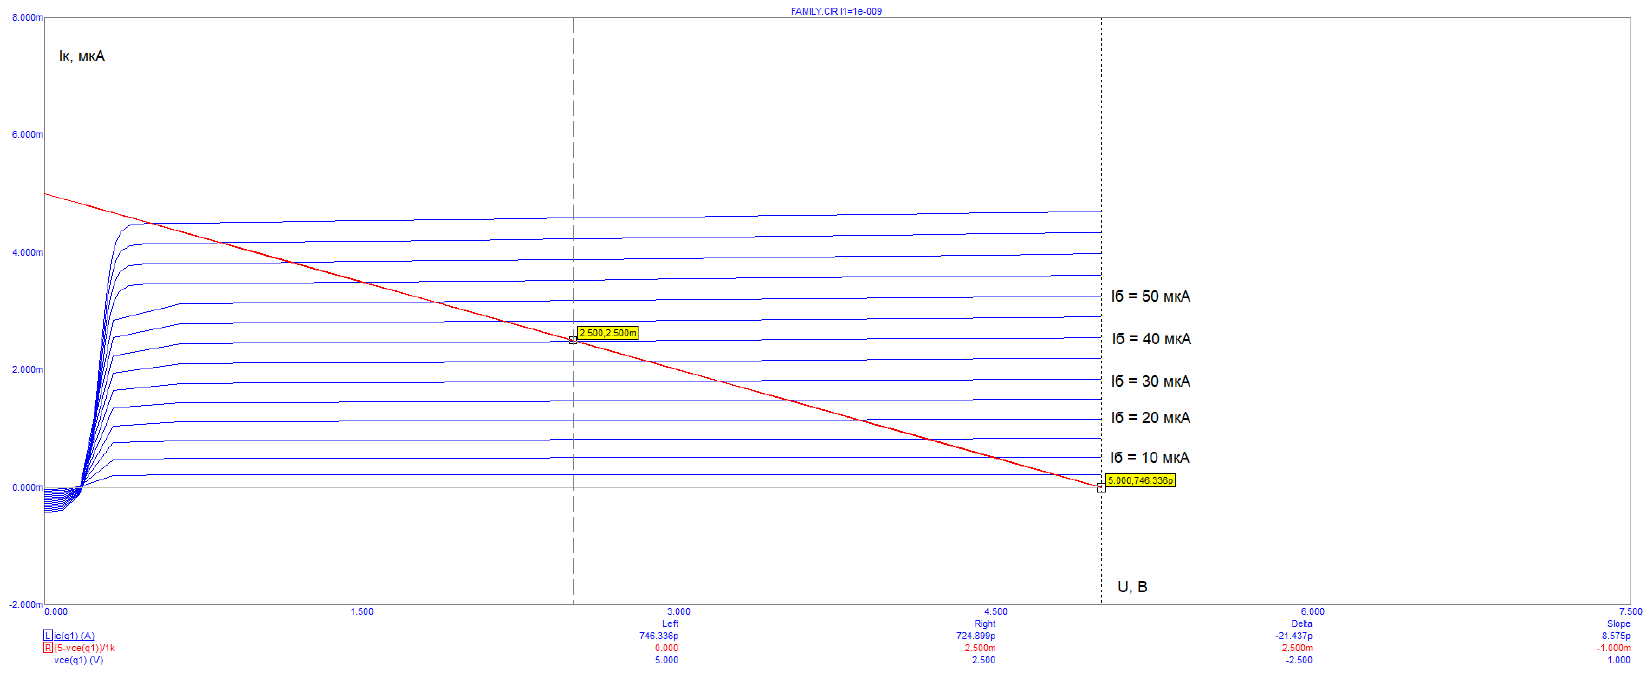
\includegraphics[width=0.9\textwidth]{graph1-4.png}
        % Підпис (зазвичай під малюнком):
        \caption{Вихідні характеристики транзистора 2N699}
        % Мітка для посилань у тексті (\ref{fig:...})
        \label{fig1-4:graph}

    \end{figure}

    На діаграмі показано вихідні характеристики транзистора 2N699, що відображають залежність колекторного струму від напруги між колектором і емітером за
    різних значень струму бази. Кожна синя крива відповідає певному фіксованому струму бази: зі зростанням цього струму збільшується і колекторний струм.
    У ділянці, де криві вирівнюються, транзистор працює стабільно, а колекторний струм майже не залежить від напруги.
    Червона лінія навантаження задає робочу точку підсилювача -- її перетин із характеристикою визначає оптимальні умови роботи схеми.

    Приймаючий, що $I_{\text{кО}} = 2{,5}$ мА, $U_{\text{кеО}} = 2{,}5$ В. Звідси знайдемо колекторний опір:

    \[
    R_{\text{к}} = \frac{E_{\text{к}} - U_{\text{кеО}}}{I_{\text{кО}}} = \frac{5 - 2{,}5}{2{,5} \cdot 10^{-3}} = 10^{3} = 1 \text{ кОм}
    \]

    \newpage

    \begin{center} \textbf{\large Аналіз схеми №2} \end{center}

    \begin{figure}[h!]

        \renewcommand{\thefigure}{\arabic{figure}} % робимо "3.1", "3.2" і т.д.

        \centering
        % Підставляєте потрібний шлях та розмір зображення:
        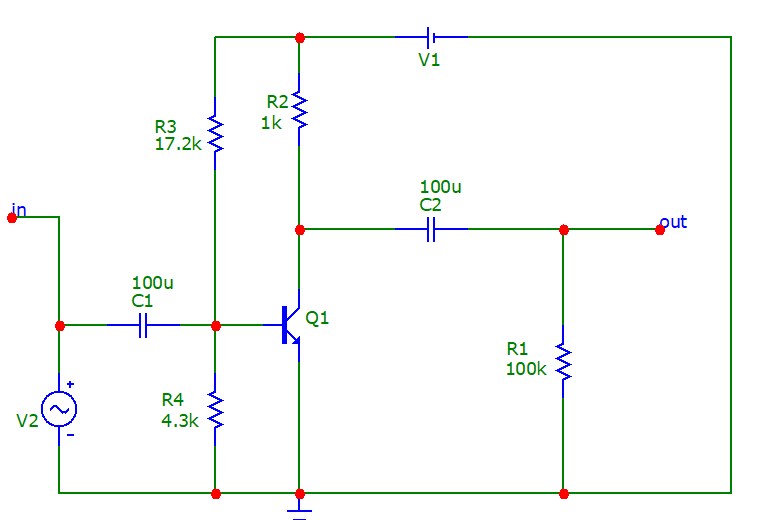
\includegraphics[width=0.5\textwidth]{scheme2-1.png}
        % Підпис (зазвичай під малюнком):
        \caption{\centering Схема однокаскадного підсилювача із фіксованою базовою напругою на біполярному транзисторі n-p-n типу}
        % Мітка для посилань у тексті (\ref{fig:...})
        \label{fig2-1:schema}

    \end{figure}

    \begin{figure}[h!]

        \renewcommand{\thefigure}{\arabic{figure}} % робимо "3.1", "3.2" і т.д.

        \centering
        % Підставляєте потрібний шлях та розмір зображення:
        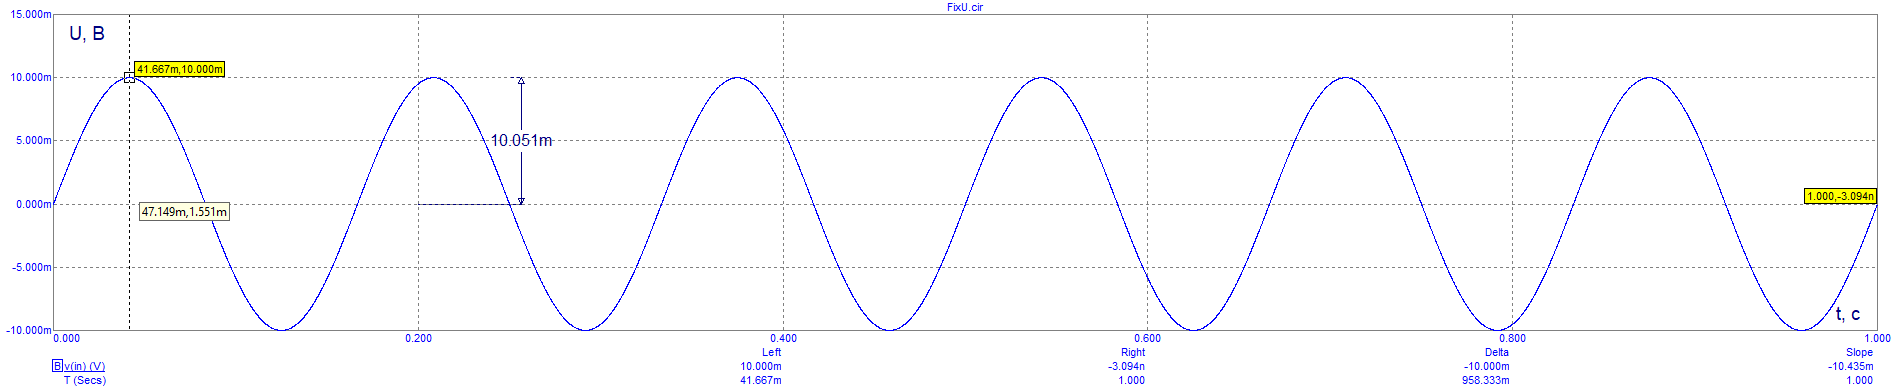
\includegraphics[width=0.7\textwidth]{graph2-1-1.png}
        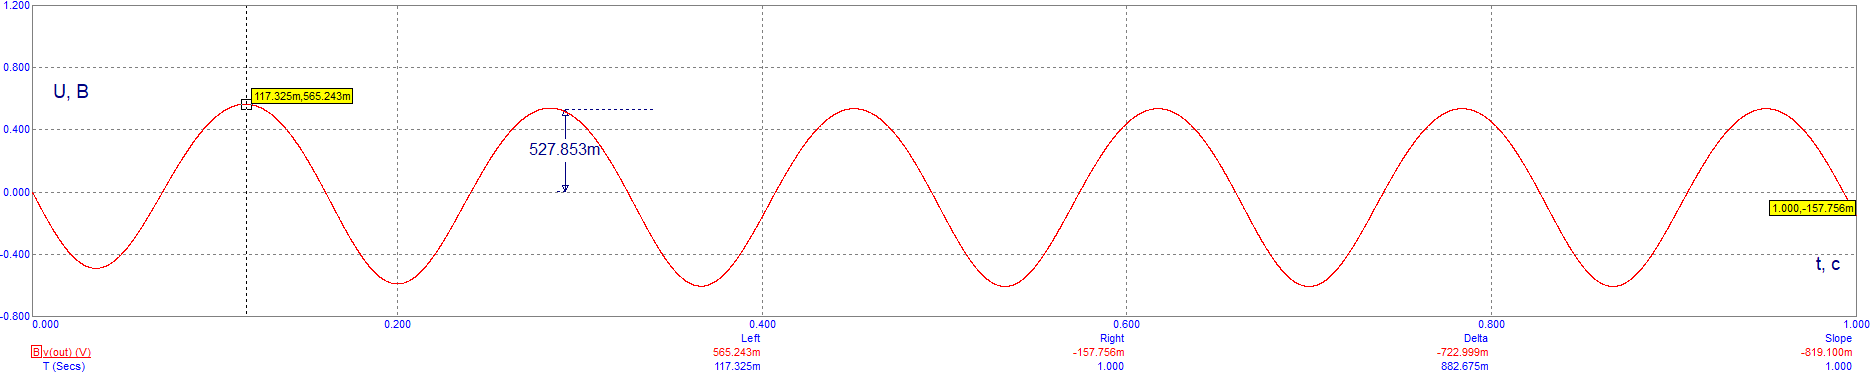
\includegraphics[width=0.7\textwidth]{graph2-1-2.png}
        % Підпис (зазвичай під малюнком):
        \caption{Часові діаграми роботи для схеми з фіксованою базовою напругою (вхід та вихід)}
        % Мітка для посилань у тексті (\ref{fig:...})
        \label{fig2-1:graph}

    \end{figure}

    Додатково маємо: $U_{out} = 565{,}243$ мВ, $U_{in} = 10$ мВ,
    $I_{\text{бо}} = 40$ мкА, $U_{\text{беО}} = 870{,}219$ мВ,
    $I_\text{п} = 5I_{\text{бо}} = 5 \cdot 40 = 200$ мкА.

    Розрахуємо значення коефіцієнта підсилення $K$ та резисторів $R_3$ і $R_4$:

    \[
    K = \frac{U_{out}}{U_{in}} = \frac{565{,}243 \cdot 10^{-3}}{10\cdot 10^{-3}} \approx 56{,}52
    \]

    \[
    R_3 = \frac{E_{\text{к}} - U_{\text{беО}}}{I_\text{п} + I_{\text{бо}}} = \frac{5 - 870{,}219 \cdot 10^{-3}}{(200 + 40) \cdot 10^{-6}} \approx 17207{,}42 \text{ Ом} \approx 17{,}2 \text{ кОм}
    \]

    \[
    R_4 = \frac{U_{\text{беО}}}{I_\text{п}} = \frac{870{,}219 \cdot 10^{-3}}{200 \cdot 10^{-6}} \approx 4351{,}09 \text{ Ом} \approx 4{,}3 \text{ кОм}
    \]

    Для визначення опору на колекторі, необхідно скористатися графіком вихідної характеристики, який ми також отримали раніше

    У нас: $U_{\text{кеО}} = 2{,}5$ В, і в цій точці $I_{\text{кО}} = 2{,}5$ мА. Звідси колекторний опір:

    \[
    R_{\text{к}} = \frac{E_{\text{к}} - U_{\text{кеО}}}{I_{\text{кО}}} = \frac{5 - 2{,}5}{2{,5} \cdot 10^{-3}} = 10^{3} = 1 \text{ кОм}
    \]

    \newpage

    \begin{center} \textbf{\large Аналіз схеми №3} \end{center}

    \begin{figure}[h!]

        \renewcommand{\thefigure}{\arabic{figure}} % робимо "3.1", "3.2" і т.д.

        \centering
        % Підставляєте потрібний шлях та розмір зображення:
        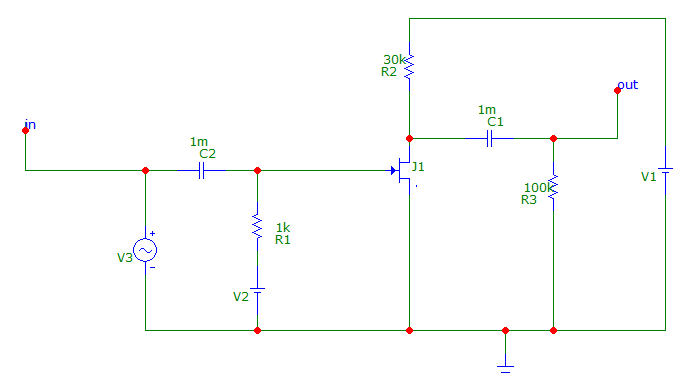
\includegraphics[width=0.5\textwidth]{scheme3-1.png}
        % Підпис (зазвичай під малюнком):
        \caption{\centering Схема із польовим транзистором з p-n-переходами та каналом n-типу}
        % Мітка для посилань у тексті (\ref{fig:...})
        \label{fig3-1:schema}

    \end{figure}

    \begin{figure}[h!]

        \renewcommand{\thefigure}{\arabic{figure}} % робимо "3.1", "3.2" і т.д.

        \centering
        % Підставляєте потрібний шлях та розмір зображення:
        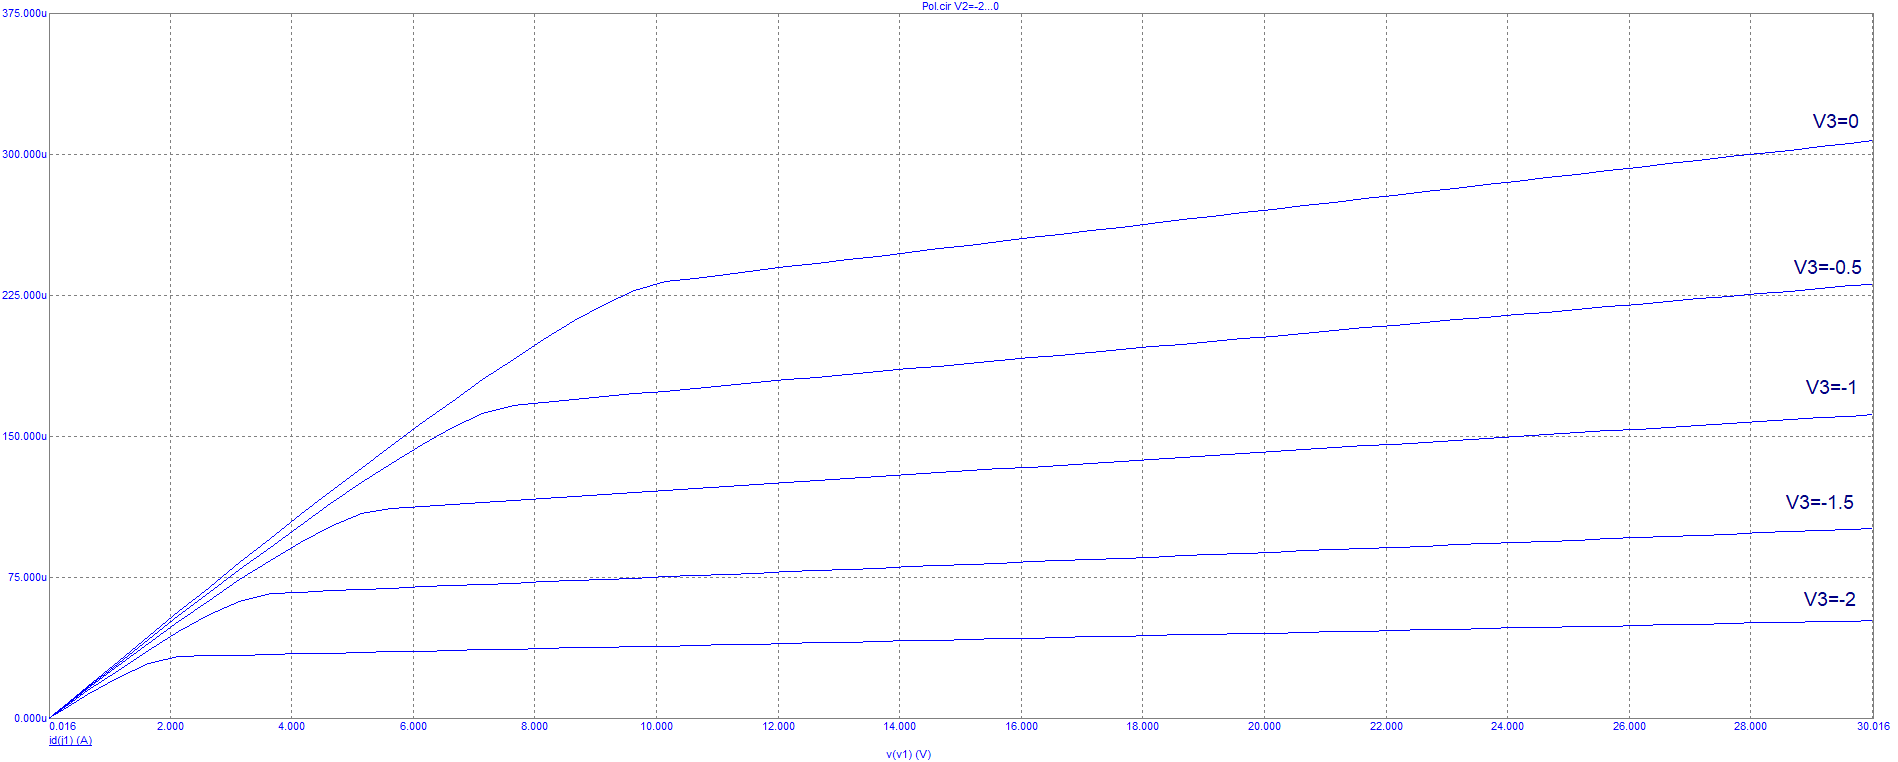
\includegraphics[width=0.7\textwidth]{graph3-1.png}
        % Підпис (зазвичай під малюнком):
        \caption{Стокові характеристики польового транзистора}
        % Мітка для посилань у тексті (\ref{fig:...})
        \label{fig3-1:graph}

    \end{figure}

    \begin{figure}[h!]

        \renewcommand{\thefigure}{\arabic{figure}} % робимо "3.1", "3.2" і т.д.

        \centering
        % Підставляєте потрібний шлях та розмір зображення:
        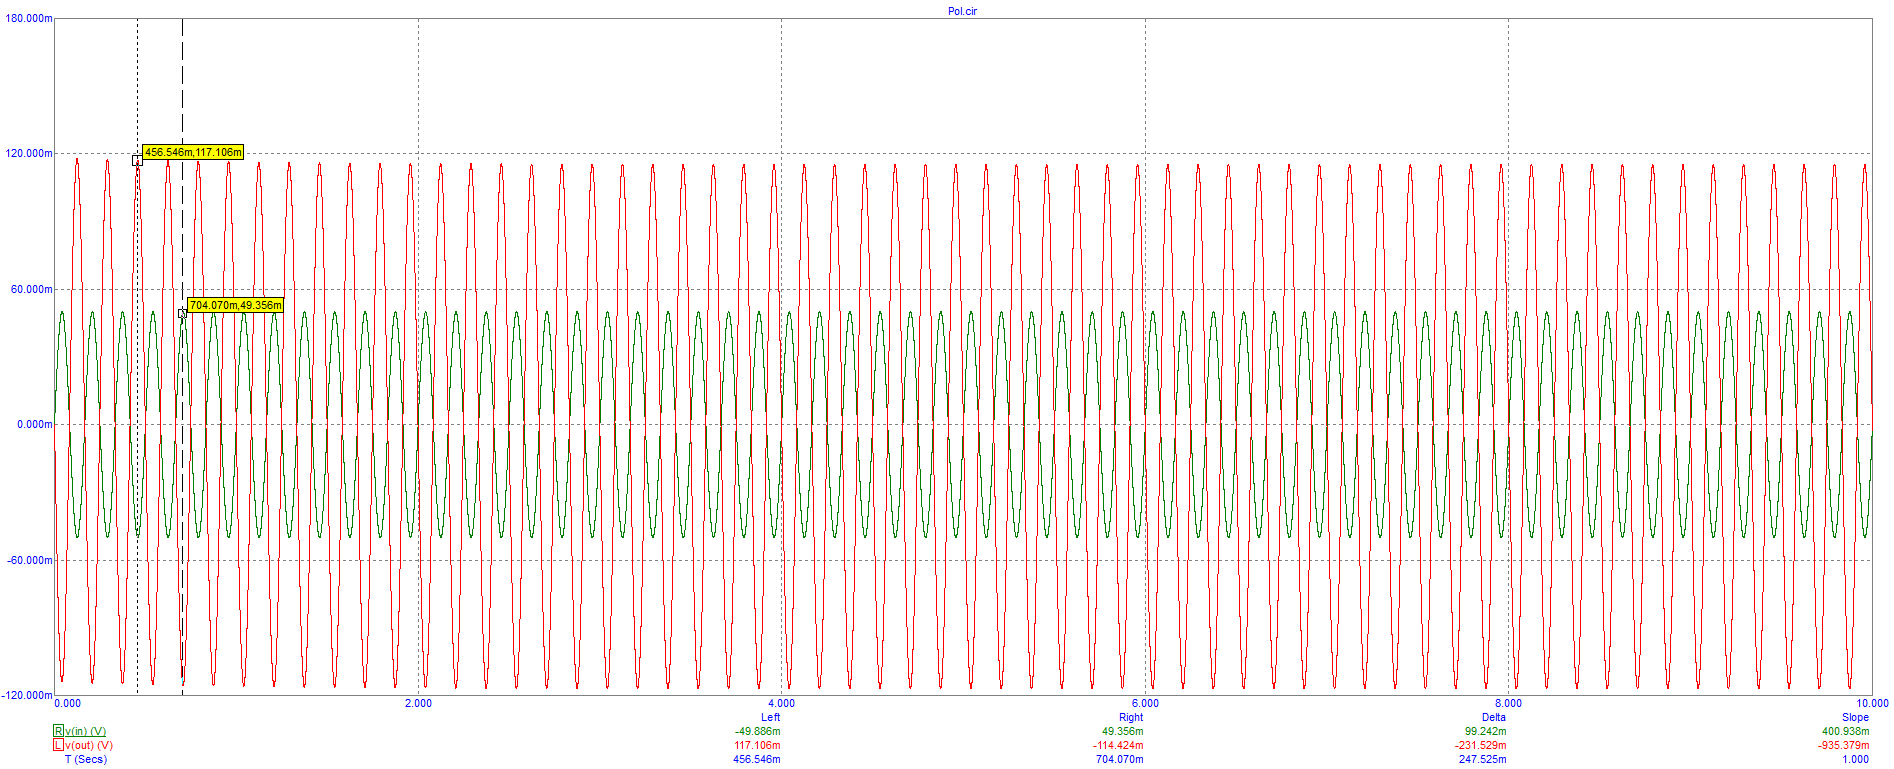
\includegraphics[width=0.9\textwidth]{graph3-2.png}
        % Підпис (зазвичай під малюнком):
        \caption{Часові діаграми роботи схеми із польовим транзистором}
        % Мітка для посилань у тексті (\ref{fig:...})
        \label{fig3-2:graph}

    \end{figure}

    У досліджуваній схемі вхідний сигнал амплітудою $\approx50$ мВ підсумовується з постійною напругою зміщення $V_2 = -1 \text{ В}$. Під час додатного півперіоду вхідного сигналу потенціал затвора стає менш від’ємним, що призводить до збільшення струму в каналі, зростання падіння напруги на резисторі $R_2$ та зменшення амплітуди вихідної напруги. При від’ємному півперіоді потенціал затвора стає більш від’ємним, струм у каналі зменшується, падіння напруги на $R_2$ зменшується, а вихідна напруга зростає. Таким чином, схема інвертує фазу вхідного сигналу на 180°.

    Крім того, амплітуда вихідної напруги перевищує амплітуду вхідного сигналу, що підтверджує підсилювальні властивості схеми. Це є типовою ознакою підсилювача на польовому транзисторі з загальним витоком, де від’ємне зміщення на затворі формує робочу точку, а змінна складова вхідного сигналу керує струмом у каналі. У результаті схема не лише підсилює сигнал, а й забезпечує його фазову інверсію, що відповідає активному режиму роботи підсилювача.

    \begin{center} \textbf{\large Аналіз схеми №4} \end{center}

    \begin{figure}[h!]

        \renewcommand{\thefigure}{\arabic{figure}} % робимо "3.1", "3.2" і т.д.

        \centering
        % Підставляєте потрібний шлях та розмір зображення:
        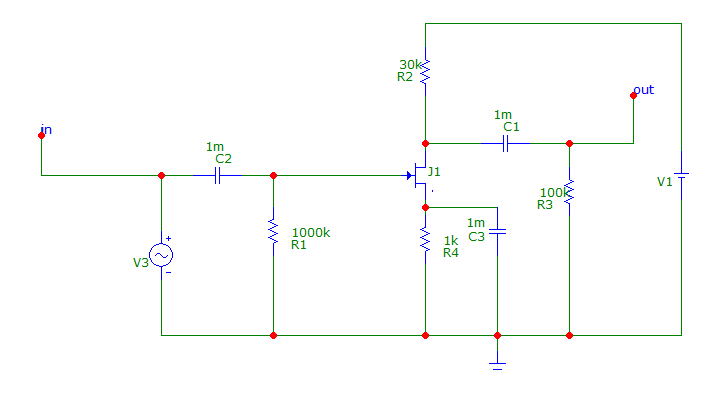
\includegraphics[width=0.5\textwidth]{scheme4-1.png}
        % Підпис (зазвичай під малюнком):
        \caption{\centering Схема підсилювача з ВЗЗна польовому транзисторі із затвором у вигляді p-n-переходу}
        % Мітка для посилань у тексті (\ref{fig:...})
        \label{fig4-1:schema}

    \end{figure}

    \begin{figure}[h!]

        \renewcommand{\thefigure}{\arabic{figure}} % робимо "3.1", "3.2" і т.д.

        \centering
        % Підставляєте потрібний шлях та розмір зображення:
        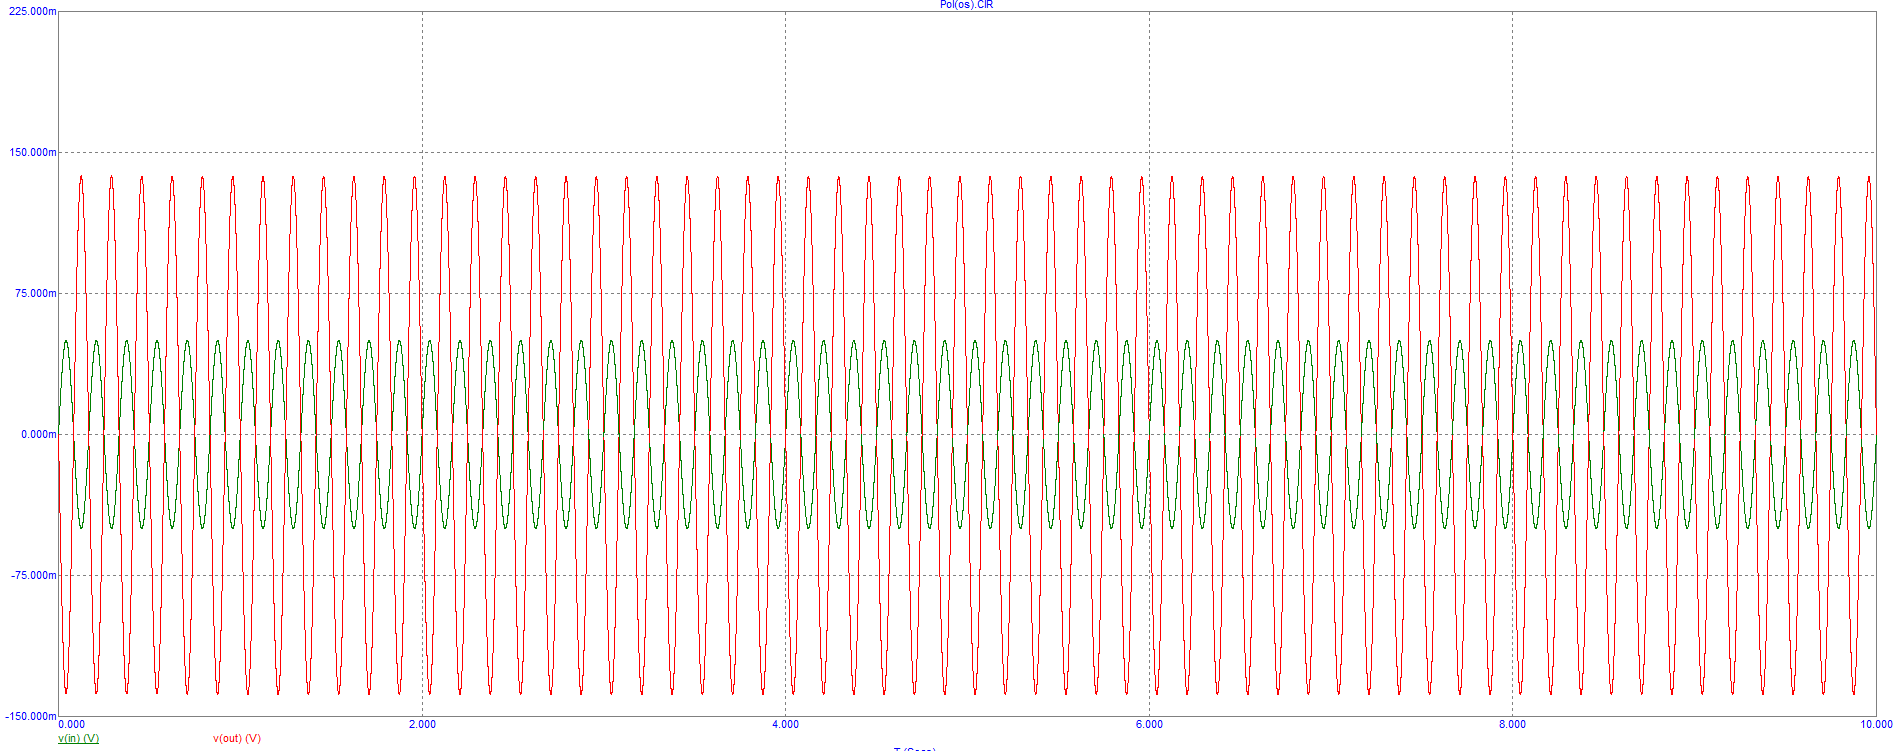
\includegraphics[width=0.9\textwidth]{graph4-1.png}
        % Підпис (зазвичай під малюнком):
        \caption{\centering Часові діаграми роботи для схеми підсилювача з ВЗЗна польовому транзисторі із затвором у вигляді p-n-переходу}
        % Мітка для посилань у тексті (\ref{fig:...})
        \label{fig4-1:graph}

    \end{figure}

    Результати моделювання підтверджують, що схема забезпечує інверсію вхідного сигналу на 180°, про що свідчить протилежна полярність вихідної напруги. При цьому амплітуда вихідного сигналу суттєво перевищує амплітуду вхідного, що вказує на ефективне підсилення. Це демонструє правильність вибору робочої точки транзистора та його стійку роботу в активному режимі.

    \newpage

    \begin{center} \textbf{\large Аналіз схеми №5} \end{center}

    \begin{figure}[h!]

        \renewcommand{\thefigure}{\arabic{figure}} % робимо "3.1", "3.2" і т.д.

        \centering
        % Підставляєте потрібний шлях та розмір зображення:
        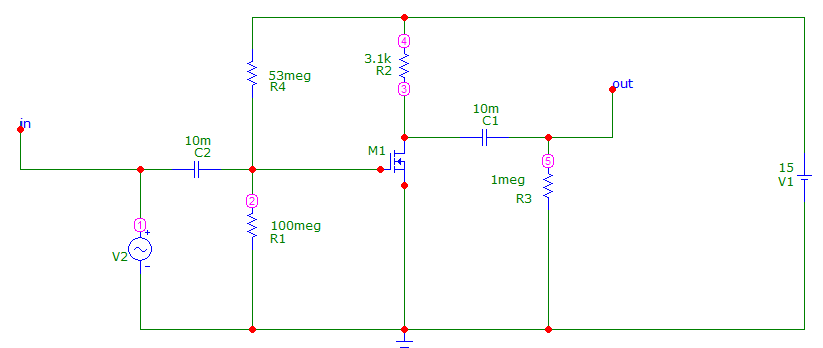
\includegraphics[width=0.5\textwidth]{scheme5-1.png}
        % Підпис (зазвичай під малюнком):
        \caption{Схема підсилювача на МОН-транзисторі з індукованим n-каналом}
        % Мітка для посилань у тексті (\ref{fig:...})
        \label{fig5-1:schema}

    \end{figure}

    \begin{figure}[h!]

        \renewcommand{\thefigure}{\arabic{figure}} % робимо "3.1", "3.2" і т.д.

        \centering
        % Підставляєте потрібний шлях та розмір зображення:
        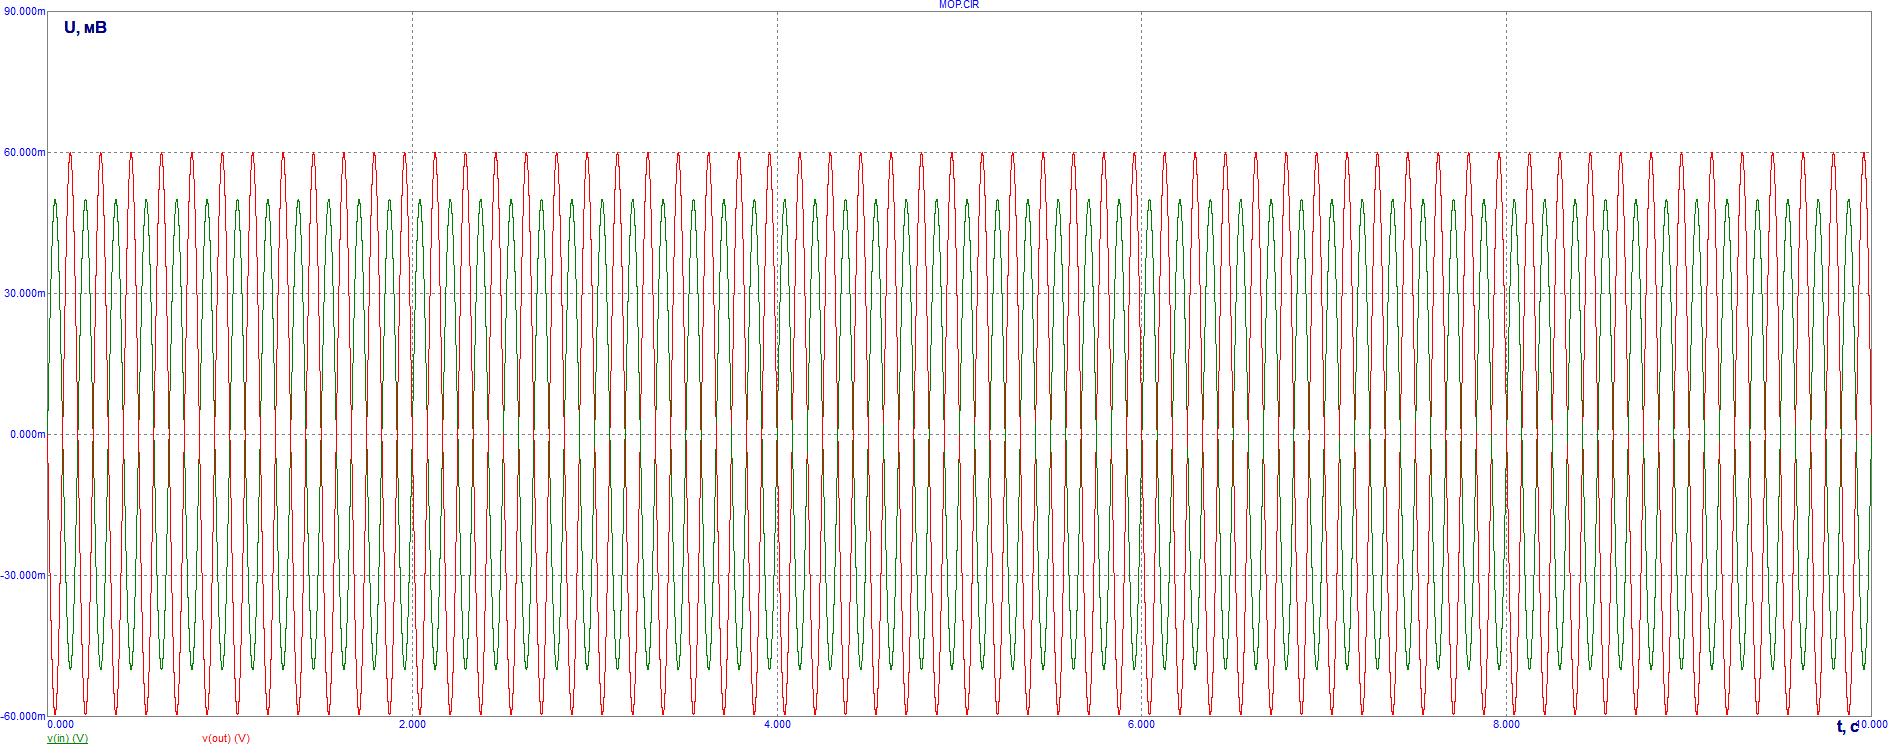
\includegraphics[width=0.9\textwidth]{graph5-1.png}
        % Підпис (зазвичай під малюнком):
        \caption{\centering Часові діаграми роботи для схеми підсилювача на МОН-транзисторі з індукованим n-каналом}
        % Мітка для посилань у тексті (\ref{fig:...})
        \label{fig5-1:graph}

    \end{figure}

    Схема реалізує підсилювач на МОН-транзисторі з індукованим каналом. Вхідна напруга подається на затвор через конденсатор, а резистивний подільник створює необхідне зміщення. Сигнал знімається з резистора у колі стоку та передається далі через розділовий конденсатор. Часова діаграма показує підсилений вихідний сигнал зі зсувом фази на 180°, що підтверджує правильну роботу підсилювача.

    \begin{figure}[h!]

        \renewcommand{\thefigure}{\arabic{figure}} % робимо "3.1", "3.2" і т.д.

        \centering
        % Підставляєте потрібний шлях та розмір зображення:
        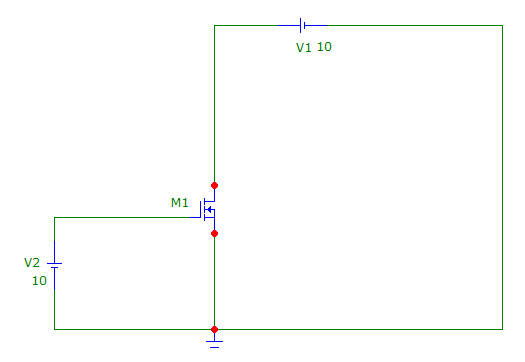
\includegraphics[width=0.5\textwidth]{scheme5-2.png}
        % Підпис (зазвичай під малюнком):
        \caption{Схема для побудови стоко-затворних характеристик МОH-транзистора DNMOS}
        % Мітка для посилань у тексті (\ref{fig:...})
        \label{fig5-2:schema}

    \end{figure}

    \newpage

    \begin{figure}[h!]

        \renewcommand{\thefigure}{\arabic{figure}} % робимо "3.1", "3.2" і т.д.

        \centering
        % Підставляєте потрібний шлях та розмір зображення:
        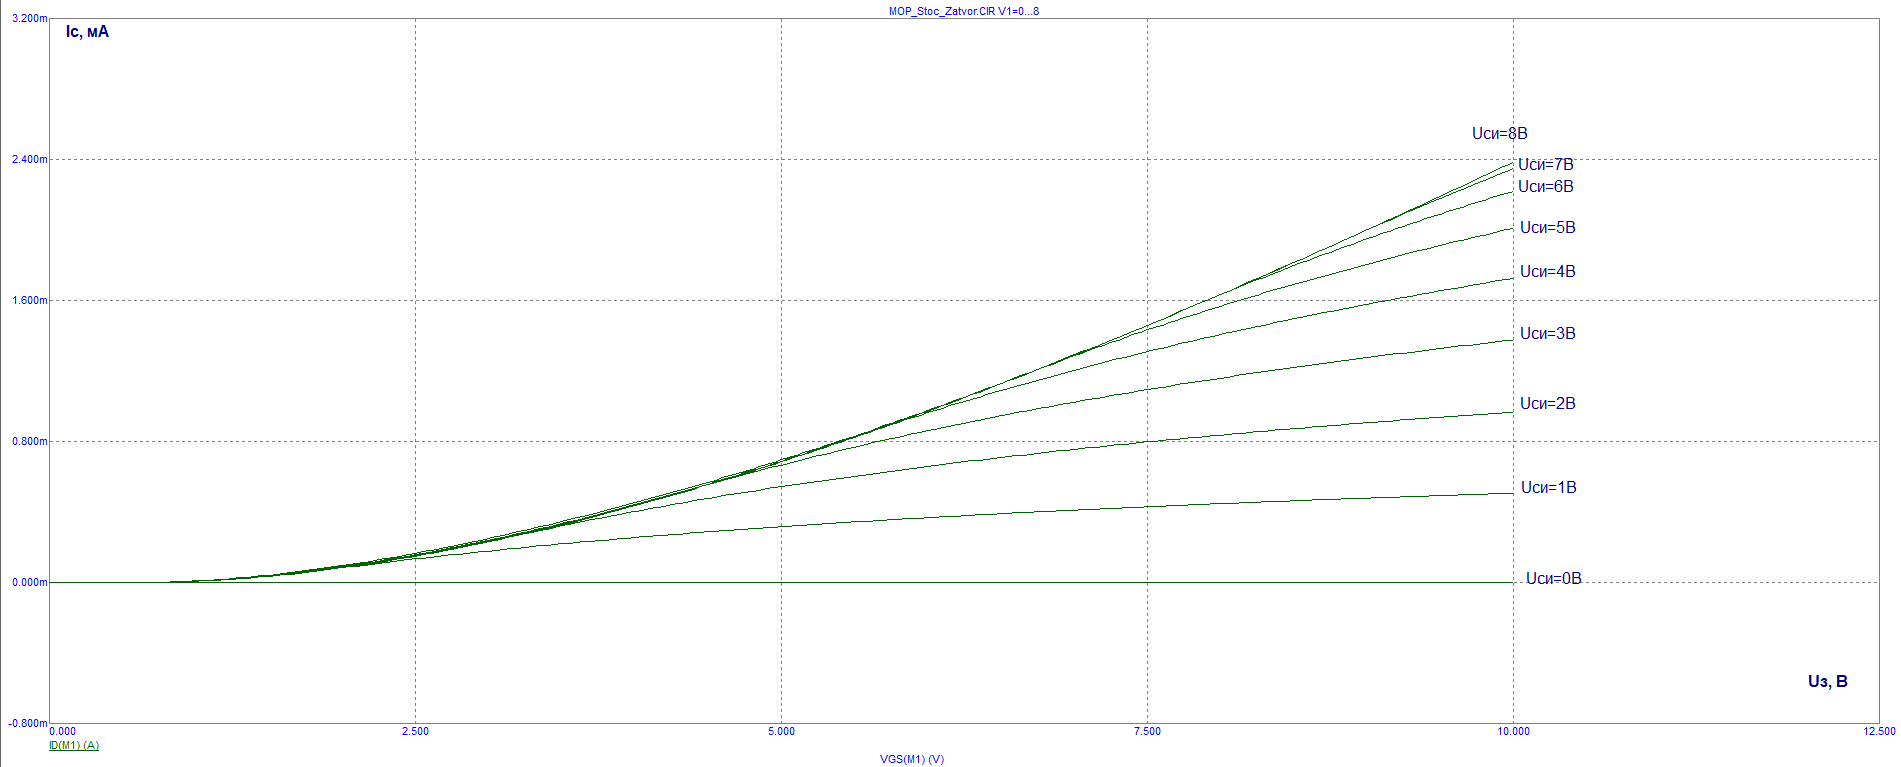
\includegraphics[width=0.9\textwidth]{graph5-2.png}
        % Підпис (зазвичай під малюнком):
        \caption{Cтокові характеристики МОH-транзистора DNMOS}
        % Мітка для посилань у тексті (\ref{fig:...})
        \label{fig5-2:graph}

    \end{figure}

    Стоко-затворні характеристики МОН-транзистора DNMOS демонструють залежність струму стоку $I_{\text{с}}$ від напруги на затворі при різних значеннях напруги сток–витік ($U_{\text{CB}}$). На графіку чітко видно порогову напругу $U_{\text{пор}}$, після досягнення якої транзистор відкривається та формується канал n-типу. Характер кривих дозволяє визначити режими роботи транзистора й обрати оптимальні умови його застосування в підсилювачах чи ключових схемах.

    \begin{figure}[h!]

        \renewcommand{\thefigure}{\arabic{figure}} % робимо "3.1", "3.2" і т.д.

        \centering
        % Підставляєте потрібний шлях та розмір зображення:
        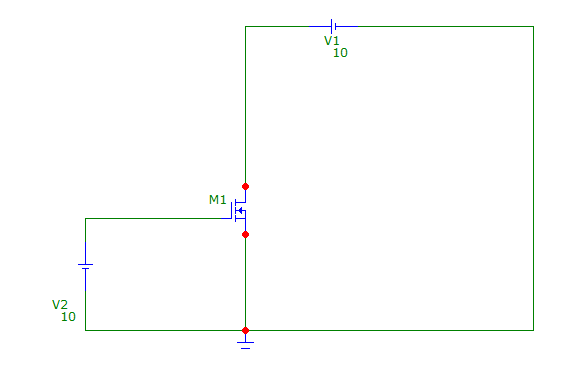
\includegraphics[width=0.5\textwidth]{scheme5-3.png}
        % Підпис (зазвичай під малюнком):
        \caption{Схема для побудови стокових характеристик МОH-транзистора DNMOS}
        % Мітка для посилань у тексті (\ref{fig:...})
        \label{fig5-3:schema}

    \end{figure}

     \begin{figure}[h!]

        \renewcommand{\thefigure}{\arabic{figure}} % робимо "3.1", "3.2" і т.д.

        \centering
        % Підставляєте потрібний шлях та розмір зображення:
        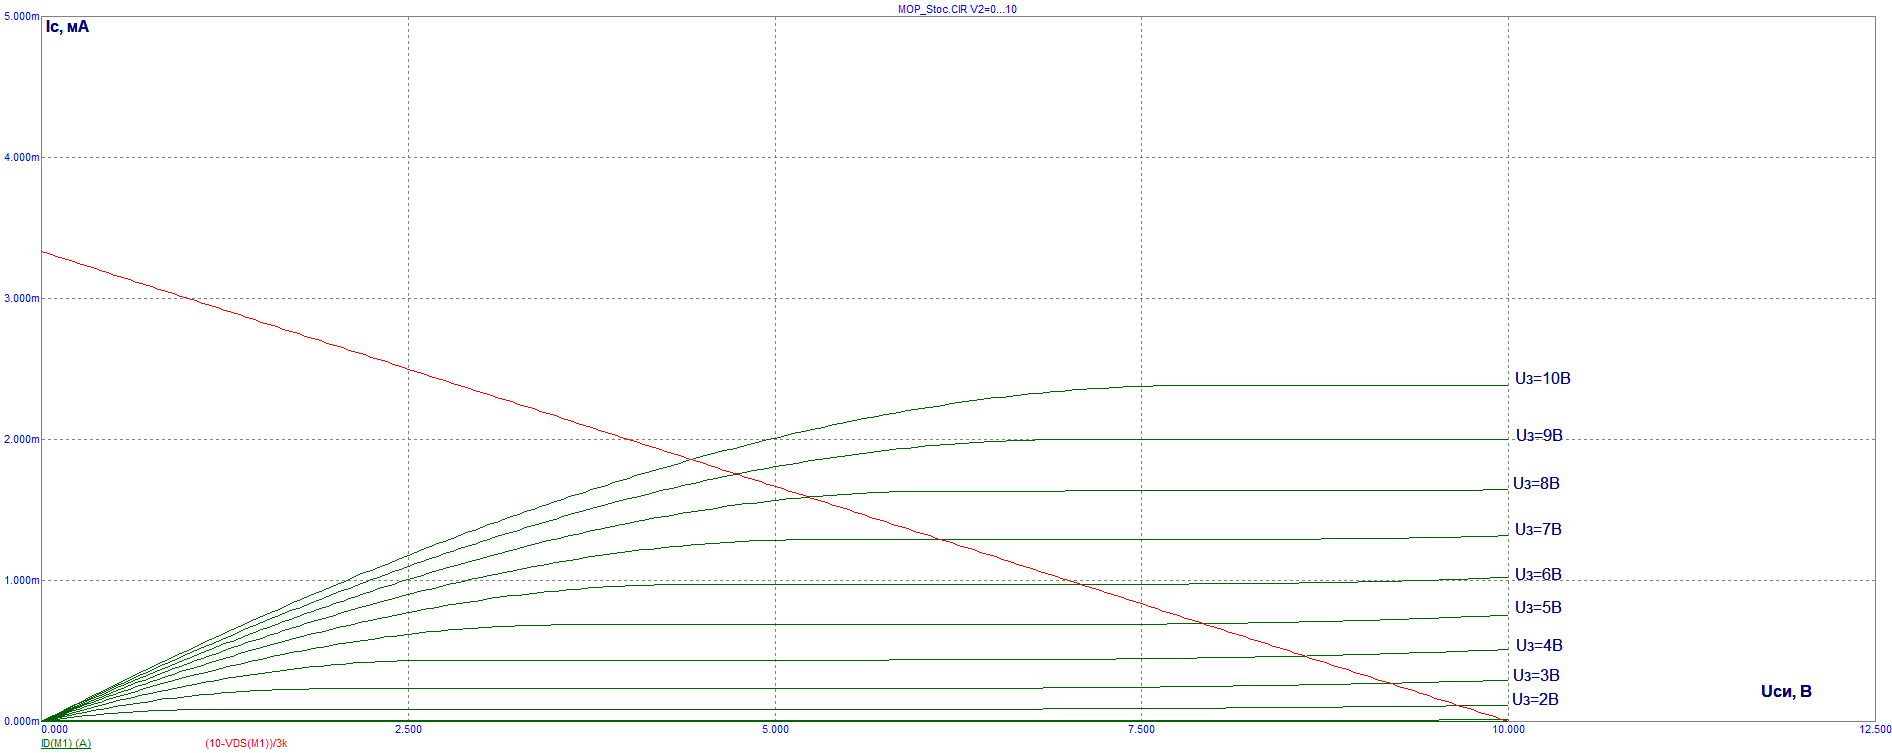
\includegraphics[width=0.9\textwidth]{graph5-3.png}
        % Підпис (зазвичай під малюнком):
        \caption{Cтоко-затворні характеристики МОH-транзистора DNMOS}
        % Мітка для посилань у тексті (\ref{fig:...})
        \label{fig5-3:graph}

    \end{figure}

    Отримані характеристики узгоджуються з теоретичними відомостями про роботу транзистора.
    Пряму навантаження будують за двома точками -- максимальною напругою на виході та максимальним струмом у колі, що дає змогу визначити робочу область і оцінити поведінку транзистора в схемі.

    \vspace{1em}

    \setlength{\parindent}{0em}

    \textbf{\underline{Висновок:}} У процесі виконання цієї лабораторної роботи я ознайомилася з принципами роботи
    підсилювальних схем на основі біполярних і МОН-транзисторів. Для біполярного транзистора було досліджено характеристики,
    визначено робочу точку та виконано розрахунки для налаштування схеми. Моделювання підтвердило наявність підсилення
    та фазового зсуву, що засвідчує правильність обраного режиму. Окрім цього, я проаналізувала характеристики МОН-транзистора
    й розглянула його режими роботи. Отримані результати відповідали теоретичним даним і сприяли набуттю практичних навичок
    роботи з електронними схемами та програмним середовищем Micro-Cap.

\end{document}